\chapter{Motivation}
\label{chapter:body}
\thispagestyle{myheadings}
\setcounter{tocdepth}{1}
% set this to the location of the figures for this chapter. it may
% also want to be ../Figures/2_Body/ or something. make sure that
% it has a trailing directory separator (i.e., '/')!
\graphicspath{{1_Intro/Figures/}}

Incoherent scatter radar (ISR) has been in use since the 1950s\cite{gordon58}.  These systems work by monitoring the reflected electromagnetic radiation from free electrons in the ionosphere.  This scatter has a specific spectral distribution from which various parameters can be determined.  Unlike other ground based measures this system can give direct measurements of various plasma parameters including electron density ($N_e$), electron temperature ($T_e$), ion temperature ($T_i$) and ion velocity ($V_i$). 

Recently the newest generation of incoherent scatter radar systems have started to come online.  These systems take advantage of phase array radar technology to give a three dimensional view to the ionosphere.  The Advance Modular Incoherent Scatter Radars (AMISR) have been developed and placed in Poker Flat Alaska and in Resolute Bay Canada.  These systems have already started to give unprecedented views in the ionosphere and upper atmosphere.  Currently EISCAT-3D is being developed as well and is expect do give even greater views due to the multi-static set up and the possibility of greater control of the phased array at even the element level.

The following section will detail the motivation of the research which is to study the high latitude ionosphere.  Examples of different types of events will given to show the dynamics of the environment. 


\section{Ionosphere and Phenomena}
The ionosphere is the area of partially ionized gas surrounding the earth and in a way is like an interface between the earth and outer space\cite{kellybook}.  The behavior of the ionosphere requires both the use of the fluid mechanics and plasma physics to describe it properly.  

The high latitude ionosphere is of special interest due to the number of different phenomena that occur in this region.  These phenomena include but are not limited to aurora borealis, polar cap plasma patches and particle precipitation events.  

The following is a listing of examples various types of high latitude ionosphere events grouped by specific behavior that is of interest the ISR sampling problem.

\begin{figure}[!t]
\centering
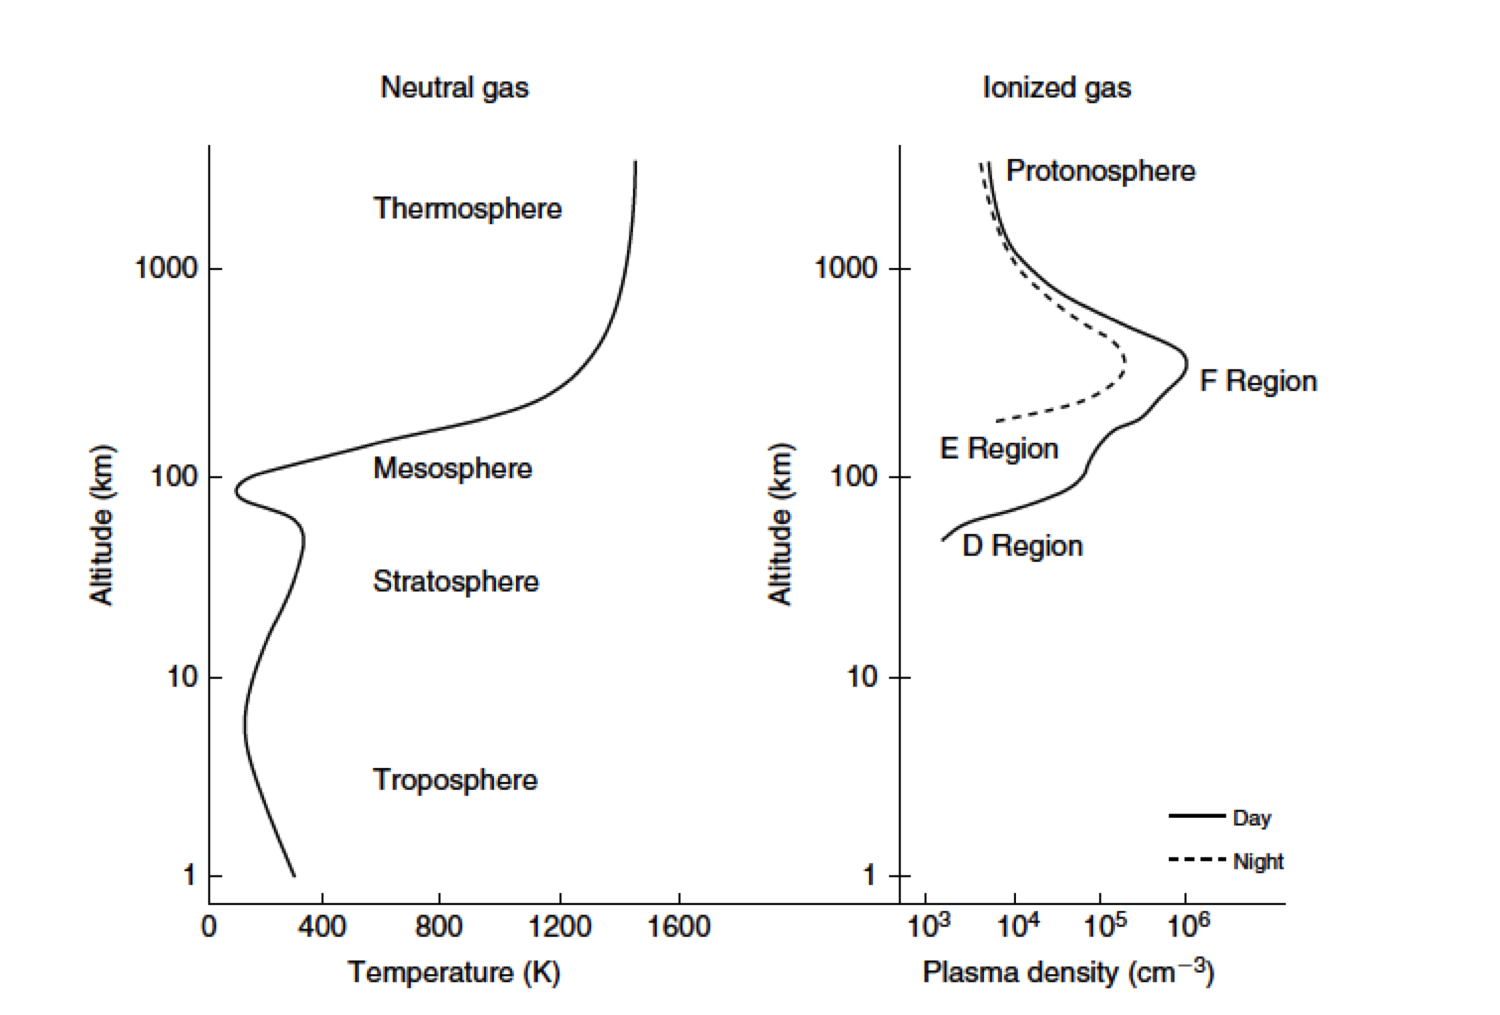
\includegraphics[width=5in]{altvsparams}
% where an .eps filename suffix will be assumed under latex, 
% and a .pdf suffix will be assumed for pdflatex; or what has been declared
% via \DeclareGraphicsExtensions.
\caption{Example profiles of neutral temperature and plasma density from \cite{kellybook}}
\label{fig:singlefilt}
\end{figure}
%These systems right now are all located in what can be considered the high latitude ionosphere.  This is a highly dynamic environment in both time and space.  The plasma can change very quickly due to the physics of the environment.  These types of events can be classified into a number of types that will be of interest to this type of sampling problem.

\subsection*{High Spatial Gradient Events}
Polar cap patches are examples where of high spatial gradients in various plasma parameters \cite{Dahlgren:2012dq},\cite{dahlgren2012di}.  In the polar cap large blobs of plasma with elevated electron density travel from the dayside to the night side ionosphere.  These patches can play a large role in plasma transport within the polar ionosphere and interfere with radio transmission as well.  Examples of sensor data that show these patches can be seen in Figure \ref{fig:patches}.

\begin{figure}[!t]
\centering
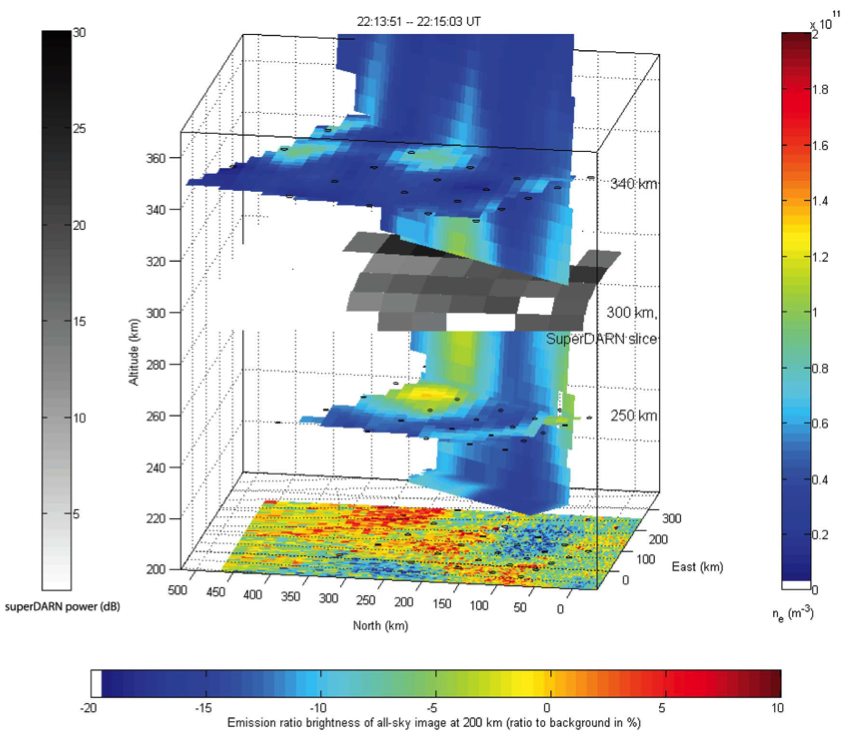
\includegraphics[width=4.0in]{patches}
% where an .eps filename suffix will be assumed under latex, 
% and a .pdf suffix will be assumed for pdflatex; or what has been declared
% via \DeclareGraphicsExtensions.
\caption{Example of polar cap patches seen in RISR and SuperDARN, from \cite{Dahlgren:2012dq}}
\label{fig:patches}
\end{figure}

Large horizontal gradients also occur during geomagnetic storms which can produce large flows.  This can create large disparities in Ion temperature as heating is occurring \cite{Zettergren:2008ba},\cite{semeter:plasmatransport2012}.  During these storms ion temperatures can go from 500$^\circ$ K to over 1500$^\circ$ K in the order of kilometers.

These high gradient events can cause some upridictible errors where two plasma population interface.  These errors can be quite complex due to the nonlinear nature of the inversion process\cite{Vallinkoski1990665}.  Similar behavior has been observed during times of auroral turbulence where shear flows seems to have caused non isotropic temperature measurements\cite{knudsen1993}. 
%\subsection*{Small Structure Events}
%\cite{semeter2010CI}
\subsection*{High Speed Events}
At times the ionosphere can be come locally unstable this can create a number of different types of turbulent events. Langmuir turbulence can create coherent structures that will be detected by ISR systems \cite{akbari:2013lt}.  These structures change on the order of one pulse repetition interval of the radar.

%Resolving these high speed events are of great interest but also a challenge.  In ISR systems each pulse is used as a sample of a spectral averaging procedure.  It is assumed that these spectrums are identical independent samples.  If spectrum changes during this time, errors in the measurement could take place.  These errors are often unpredictable due to the nonlinear fitting used to fit the spectrum with the plasma parameters.
 %\cite{Dahlgren:2013ip}
%In the past researchers have studied errors associated with different plasma distributions mixing together.  These errors can be quite complex due to the nonlinear nature of the inversion process\cite{Vallinkoski1990665}.  Similar behavior has been observed during times of auroral turbulence where shear flows seems to have caused non isotropic temperature measurements\cite{knudsen1993}. 
\section{ISR Sampling}
For this prospectus we will be proposing to improve the spatial and time sampling of the ISR systems.  New phase array radar systems have allowed for an unprecedented amount of flexibility in sampling the environment.  As such there has been no optimal way developed as of yet to sample this space.  Currently ISR systems integrate their spectral estimate in time only.  In order to get a statistical desirability of their measurements these systems may have to integrate for a long period of time.  It may be possible to integrate across different beams if stationarity can be found.  Other techniques could also be investigated such as well to try to improve the ISR measurements.

In this prospectus we will present the methodology with which ISR performs the measurement of the plasma parameters.  This will be done to show possible methods for improving the technique.